%! Author = joels
%! Date = 24/12/2020

\section{Sequences and Iterators}
% You can use std array and std vector in your code
% You can use an iterator to access container elements
% You can access and modify container contents using algorithms
% You can interact with streams through iterators

\subsection{Std::array and std::vector}
\subsubsection{Array}

\begin{itemize}
    \item C++'s std::array$<$T, N$>$ is a fixed size Container
        \SubItem{T is a template type parameter. N is a positive integer parameter}
    \item std::array can be initialized with a list of elements 
        \SubItem{The size of an array must be known at compile time and cannot be changed}
        \SubItem{Otherwise it contains N default constructed elements: \textcolor{blue}{std::array$<$int, 5$>$ emptyArray}}
    \item The size is bound to the array object and can be queried using \textcolor{blue}{.size()}
    \item Avoid plain C Array whenever possible: \textcolor{red}{int arr [ ]$\{$1, 2, 3, 4, 5$\}$;}
\end{itemize}
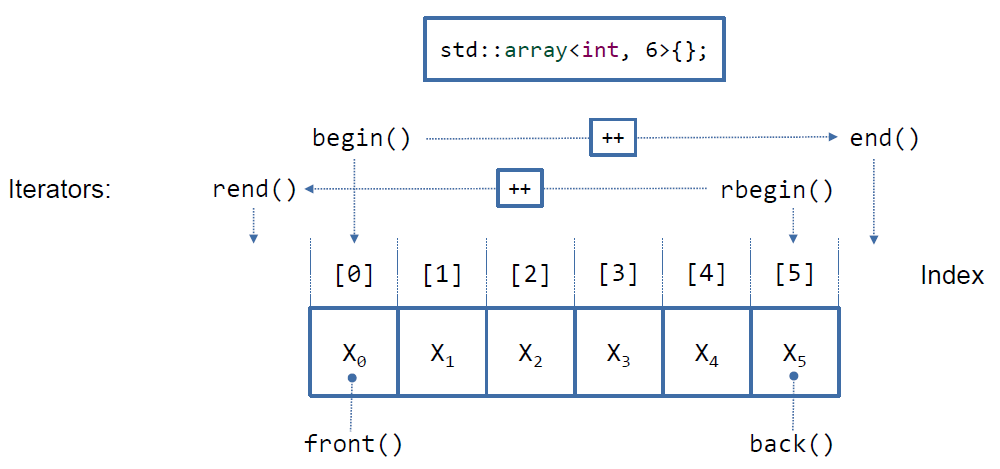
\includegraphics[scale=0.46]{array_iterators}
\subsubsection{Vector}
\begin{itemize}
    \item C++'s std::vector$<$T$>$ is a Container: contains its elements of type T (no need to allocate them)
        \SubItem{java.util.ArrayList$<$T$>$ is a collection = keeps references to T objects}
        \SubItem{T is a template parameter}
    \item std::vector can be initialized with a list of elements
        \SubItem{Otherwise it is empty: \textcolor{blue}{std::vector$<$double$>$ vd$\{$ $\}$;}}
        \SubItem{Other construction means might need parentheses (legacy)}
    \item When an initializer is given, the element type can be deduced! \textcolor{blue}{std::vector$\{$1, 2, 3, 4, 5$\}$;}
\end{itemize}
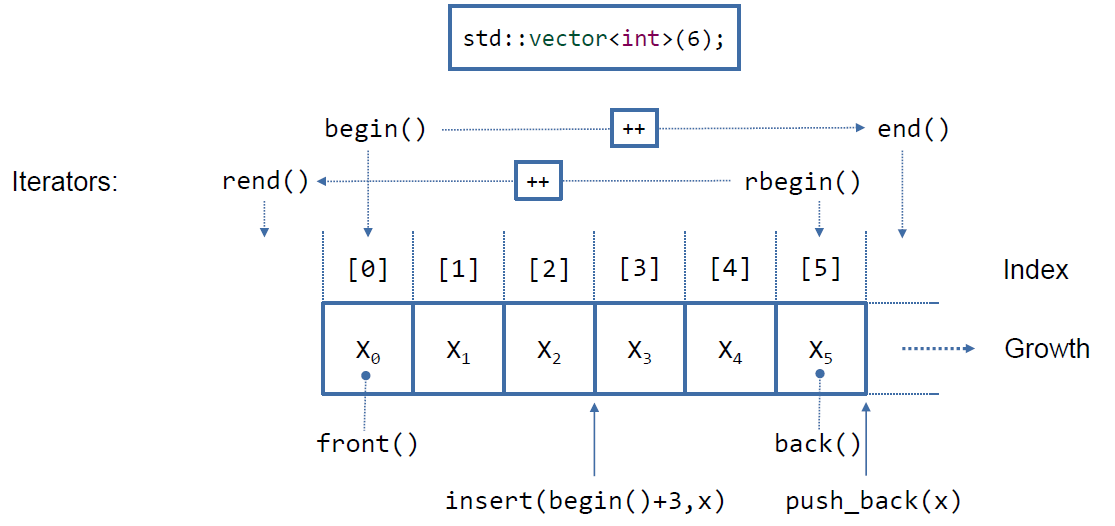
\includegraphics[scale=0.46]{vector_iterators}\\
Parenthesis at definition allow providing initial size, when type of elements is a number:\\
\textcolor{blue}{std::vector$<$string$>$ words$\{$6$\}$;} $\rightarrow$ Um sicher zu gehen die Grösse mit runden Klammern angeben.\\

\textbf{Für beide Datentypen:}\\
Element access using subscript operator [ ] or at():\\
at throws an exception and [ ] has undefined behavior on invalid access.\\

\textbf{Speicherort:}\\
Generell werden alle Elemente einer Klasse auf dem Stack abgelegt. So auch der Vector. Fügt man dem Vector ein Element hinzu, wird davon eine unabhängige Kopie auf dem Heap erstellt. Der Vector referenziert auf das neue Objekt.

\subsection{Iteration}
\subsubsection{Element Iteration (Range-Based for-Loop)}
\begin{center}
    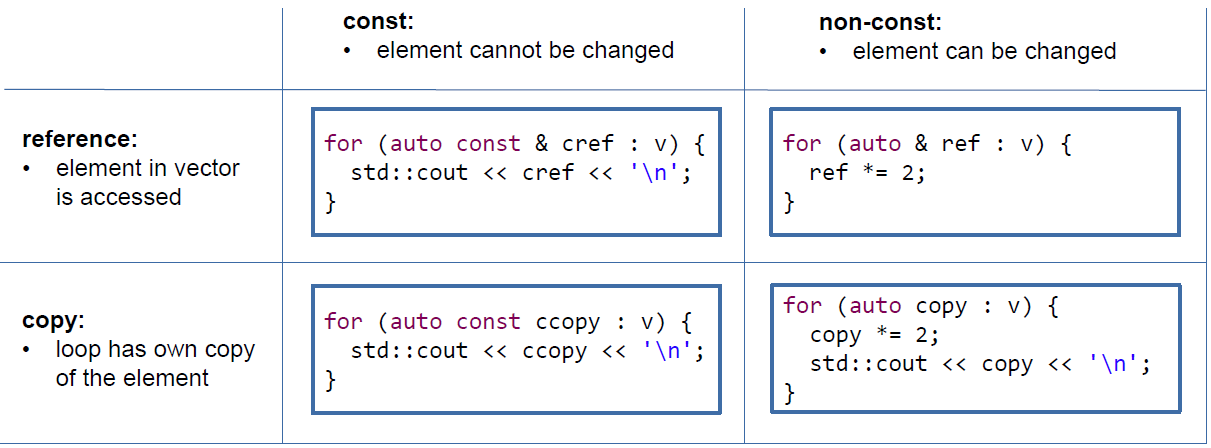
\includegraphics[scale=0.5]{range_based_for_loop.png}
\end{center}
\subsubsection{Iteration with Iterators}
\begin{lstlisting}[style=frame, style= linenumbers, language=C]
// Changing the element in a non-const container is possible in this way
for (auto it = std::begin(v); it != std::end(v); ++it) {
    std::cout << (*it)++ << ", "; }
// Guarantee to just have read-only access with std::cbegin() and std::cend()
for (auto it = std::cbegin(v); it != std::cend(v); ++it) {
    std::cout << *it << ", "; }
\end{lstlisting}

\subsection{Iterators with Algrotithms}
\begin{lstlisting}[style=frame, style= linenumbers, language=C]
// Counting values: std::count
size_t count_blanks (std::string s) {
    return std::count(s.begin(), s.end(), ' '); }

// Summing up all values in a vector: std::accumulate
std::vector<int > v{5, 4, 3, 2, 1};
std::cout << std::accumulate(std::begin(v), std::end(v), 0) << " = sum\n";

// Number of elements in range: std::distance
void printDistanceAndLength (std::string s) {
    std::cout << "distance: " << std::distance(s.begin(), s.end()) << '\n';
    std::cout << "in a string of length: " << s.size() << '\n';
}

// std::for_each
void printAll(std::vector<int> v) {
    std::for_each(crbegin(v), std::crend(v), print); }

// std::for_each with Lambda
void printAll(std::vector<int> v, std::ostream & out) {
    std::for_each(crbegin(v), std::crend(v), [&out](auto x) {
        out << "print: " << x << '\n';
    }); }

// std::copy (target needs to be an iterator too. target.end() would not work)
std::vector<int> source{1, 2, 3}, target{};
std::copy(source.begin(), source.end(), std::back_inserter target(target));

// Filling a vector with std::fill
std::vector<int> v(10);
std::fill(std::begin(v), std::end(v), 2);
// Or even easier:
std::vector v(10, 2);

// std::generate()
std::vector<double> powerOfTwos(5);
double x{1.0};
std::gegerate(powerOfTwos.begin(), powerOfTwos.end(), [&x] {return x *= 2.0; });
// std::generate_n
std::vector<double> powerOfTwos();
double x{1.0};
std::gegerate(std::back_inserter(powerOfTwos), 5, [&x] {return x *= 2.0; });

// fills a range with subsequent values (1,2,3,...): std::iota()
std::vector<int> v(100);
std::iota(std::begin(v), std::end(v), 1);

// std::find(), std::find_if() - If no match exists the end of the range is returned
auto zero_it = std::find(std::begin(v), std::end(v), 0);
if (zero_it == std::end(v)) { std::cout << "no zero found \n"; }
// std::count_if()
std::cout << std::count_if(begin(v), end(v), [](int x) { return isEven(x); }) << " even numbers\n";
\end{lstlisting}

\subsection{Iterators for I/O}
\begin{itemize}
    \item std::ostream\_iterator$<$T$>$
        \SubItem{outputs values of type T to the given std::ostream}
        \SubItem{No end() marker needed for ouput, it ends when the input range ends}
    \item std::istream\_iterator$<$T$>$
        \SubItem{reads values of type T from the given std::istream}
        \SubItem{End iterator is the default constructed std::istream\_iterator$<$T$>$$\{$$\}$}
        \SubItem{It ends when the Stream is no longer good()}
\end{itemize}
\subsubsection{Shorter types with the keyword using.}
\begin{lstlisting}[style=frame, style= linenumbers, language=C]
// Copy Strings from standard input to standard output
// Skips white space !!
using input = std::istream_iterator<string>;
input eof{};
input in{std::cin};
std::ostream_iterator<string> out{std::cout, " "};
std::copy(in, eof, out);

// std::istreambuf_iterator<char> uses std::istream::get to get every character
// Only works with char-like types
using input = std::istreambuf_iterator<char>;
input eof{};
input in{std::cin};
std::ostream_iterator<char> out{std::cout, " "};
std::copy(in, eof, out);

// Fill a vector from a stream (copy with back_inserter)
using input = std::istream_iterator<int>;
input eof{};
std::vector<int> v{};
std::copy(input{std::cin}, eof, std::back_inserter(v));

// Fill a vector from a stream (directly rom two iterators)
using input = std::istream_iterator<int>;
input eof{};
std::vector<int> const v{input{std::cin}, eof};
\end{lstlisting}

